%%%%%%%%%%%%%%%%%%%%%%%%%%%%%%%%%%%%%%%%%%%%%%%%%%%%%%%%%%%%%%%%%%%%%%%%%
%
% Purpose: Specification for JSC Engineering Orbital Dynamics (JEOD)
%
%
%
% 
%%%%%%%%%%%%%%%%%%%%%%%%%%%%%%%%%%%%%%%%%%%%%%%%%%%%%%%%%%%%%%%%%%%%%%%%%

\chapter{Product Specification}\hyperdef{chapter}{spec}{} \label{ch:spec}
\section{Conceptual Design}
\subsection{Features and Linage of JEOD}
 JSC Engineering Orbital Dynamics (JEOD) is a collection of computational mathematical models that provide vehicle or vehicles trajectory generation by the solution of a set of dynamics models represented as differential equations.  The orbital dynamics models that now comprise JEOD were part of the Trick Simulation Development Environment since its inception in the early 1990s.  These models have found wide use in many simulations across NASA's Johnson Space Center.  Some of these simulations have been used for Space Shuttle and International Space Station mission support.  In that capacity, they have a significant lineage and have developed a level of credibility in the space operations environment that is essential to these space flight programs and more broadly valued by the agency.

It is important to note that these space flight programs are restricted to an orbital regime referred to as Low Earth Orbit (LEO - between 160 - 2,000 km (100 - 1,240 miles) above the Earth's surface).  As a result, the Trick orbital dynamics package was originally designed for use and tested in that orbital regime.  However, NASA has a history and now a renewed vision to explore beyond LEO and JEOD has expanded to be an orbital dynamics package that supports those regimes.

Three fundamental areas are essential to the design of JEOD and they are:
\begin{itemize}

\item Coordinate systems and reference frames,

\item Time standards and time scales, and

\item Multi-vehicle dynamics.

\end{itemize}

Of these three fundamental focus areas, the multi-vehicle dynamics area is fundamentally dependent on the time and coordinate frames areas.  However, even time and coordinate frames are interdependent to some level, depending on the underlying assumptions of the dynamics.  In the following few paragraphs, we discuss JEOD design and capabilities of each of these areas.

Since a key objective for JEOD is to provide support for exploration missions, it needs to allow for multiple planetary and interplanetary reference frames.  In addition, the requirement for multi-vehicles about multiple planets meant no single reference frame choice was possible. Even though the solar system barycenter frame might be one potential candidate for a central reference frame, it is numerically undesirable to propagate the state of a vehicle orbiting Neptune in this frame.  Therefore, JEOD is implemented to use a reference frame tree concept.  This provides a framework for associating dynamical reference frames consistently and efficiently.  For more detailed information on the coordinate systems modeling in JEOD, see the \hypermodelref{REFFRAMES}\ and \hyperCoordFrame\ documentation.

The JEOD time model supports the concept of a dynamic time that is linearly tied to simulation executive step time, but is not required to step forward in a 1 second to 1 second dependancy.  This increases the accuracy (some would argue correctness) of the time model, and allows for JEOD dynamic time move backward if needed.  The JEOD time model is an extensible object oriented model, which supports the concepts of time standards that can be extended by the user.  These time standards can have varying rates of propagation with respect to the base dynamic time.  For more detailed information on the time model, see the \hypermodelref{TIME}\ documentation.

The final foundation area is multi-vehicle dynamics and JEOD is designed to efficiently and accurately propagate multiple vehicles about multiple planets. while allowing for interactions between said vehicles.  This dynamic infrastructure depends on both the reference frames model and the time model discussed above.  For more information on the multi-vehicle dynamics model, see the \hypermodelref{DYNBODY} , \hypermodelref{DERIVEDSTATE} , \hypermodelref{DYNMANAGER} , \hypermodelref{MASS}\ documentation.

While other areas are also important to the successful implementation of an orbital dynamics package, these three form the foundation upon which the others are built.  In addition to the purely technical issues associated with modeling physical orbital dynamical systems in a digital computational environment, there are also the software architecture or design challenges associated with the practical constraints of computer languages, operating systems and platforms.  So, in addition to supporting the technical base of JEOD, the JEOD team focuses on what are sometimes referred to as software ``ilities".  The definition of ``ilities" varies from reference to reference but often includes concepts like the following: reliability, security, scalability, extensibility, manageability, maintainability, interoperability, composability, evolvability, survivability, affordability, understandability, and agility.

JEOD continues to maintain as much of the pedigree and usage history of JEOD and its historical software base, but is now designed using modern and extensible computational constructs (e.g. extensibility, generalization, data encapsulation, etc.).  The original Trick based dynamics packages were written in the C programming language (including JEOD 1.4 and 1.5), and the current version of JEOD is written in the C++ programming language.  The principal benefits in this choice are that C is, for the most part, a subset of C++ so older models were easily converted and that C++ supports the object oriented programming constructs deemed necessary for a modern design.

\begin{table}[h!]
\begin{center}
\caption{JEOD Features} \vspace{5mm} \label{tbl:benifits}
\begin{tabular}{||c||p{9cm}||} \hline
{\bf JEOD Feature}  \\ \hline \hline
{\bf Reference Frame Model} & {A well-formulated model of reference frames and operations on them.  Reference frames are organized in a tree structure, with the International Celestial Reference Frame at the root of the tree.}  \\ \hline \hline
{\bf Multiple Integration Frames} & {Each independent body in a simulation has its own integration frame. This capability is essential for a multi-vehicle simulation in which one vehicle orbits one planet such as the Earth while another vehicle orbits the a different planet such as the Moon.}  \\ \hline \hline
{\bf Time Representations Model} & {A flexible and extensible model of time.}  \\ \hline \hline
{\bf Body Actions Model} & {A flexible and extensible mechanism for initializing and asynchronously operating on vehicle objects.}  \\ \hline \hline
{\bf Derived States} & {A flexible and extensible mechanism for computing information that derives from vehicle states.  The Body Action and Derived State models are designed for extensibility.  Suppose you don't like the limited set provided with JEOD. Fine! Make the one that you like. It's easy.}  \\ \hline \hline
{\bf MassBody/DynBody} & {Mass and OrbitalBody objects that take full advantage of inheritance allowing users to extend this inheritance even further. For example, JEOD uses the rigid body assumption, a user-defined derived class could eliminate this.}  \\ \hline \hline
{\bf Surfaces Model} & {Allows the modeling of environmental effects such as aerodynamic drag, radiation pressure, contact and articulation.}  \\ \hline \hline
{\bf JEOD Tutorial} & {The Tutorial takes the JEOD user from very simple simulations to the more complex, in a well-ordered progression.}  \\ \hline \hline
{\bf C++ Language} & {The entire JEOD Software Package is written in the C++ language, which allows users to develop their own models by simply extending JEOD base classes.}  \\ \hline \hline
{\bf Software Documentation} & {All JEOD models are documented in a concise and consistant manner.}  \\ \hline \hline
\end{tabular}
\end{center}
\end{table}

\newpage\subsection{Reference Documents}
The following documents provide supporting reference material for understanding the orbital dynamics concepts that have been implemented in JEOD:
\begin{itemize}
\item Vallado,"D.A. Vallado with tech contributions by Wayne D. McClain" \cite{VMcC}
\item Montenbruck and Gill, "Satellite Orbits" \cite{MG}
\item Hughes,  "Spacecraft Attitude Dynamics" \cite{Hughes}
\item Bate, White and Mueller, "Fundamentals of Astrodynamics" \cite{BMW}
\item Seidelmann, "Explanatory Supplement to the Astronomical Almanac" \cite{Seidelmann}
\item Heafner, "Fundamental Ephemeris Computations for use with JPL data" \cite{Heafner}
\end{itemize}

See the bibliography for the details associated with these references.

\section{Detailed Design}
\subsection{JEOD Root Directory}
The top level or JEOD root directory is organized into several subdirectories as follows:
\begin{itemize}
\item bin - Scripts to facilitate JEOD use,
\item docs - Contains this document and all other JEOD-wide references or documentation,
\item models - Divided into four sections (dynamics, environment, interactions, utils) which contain the functional parts of JEOD referred to as models,
\item sims - Example simulations such as the JEOD Tutorial,
\item verif - Verification simulations and data.
\end{itemize}

\subsection{A JEOD Model}\label{desc:modeldesc}
A JEOD model is a cohesive, related (i.e., not random) collection of C++ classes.  It is also an immediate subdirectory of one of the four major model category directories; dynamics, environment, interactions, and utils.  Each model is a directory and a directory is a model.  This ensures that the contents of a model directory are truly related and that all components of a model are located in a single directory.

Each model directory can contain the following subdirectories.
\begin{itemize}
\item docs - Model documentation,
\item data - Data files, suffix .d or .hh and .cc if an initialization class,
\item include - Header files, suffix .hh,
\item src - Implementation files, suffix .cc,
\item verif - Verification files and simulations, typically organized in subdirectories, i.e.. SIM\_...,
\end{itemize}

In some cases it makes sense to break a model into smaller parts, so a few JEOD models contain sub-models.  These sub-models obey the same basic concepts used for models.  They are reasonably self-contained (e.g., a class), separated in only one subdirectory, and consist of logically consistent parts.  Each sub-model will contain an include and src subdirectory in addition to any others that are required, such as data or verif.

\subsection{Model Categories}
As a matter of basic design and organization, the models that comprise JEOD are divided into four categories.  This organization was introduced in Chapter \ref{ch:intro}, and below is a table showing all the models in JEOD and the category they belong too.  Each model name in the table is a hyperlink to the individual model document.

\begin{table}[h!]
\begin{center}
\caption{JEOD Model Tree} \vspace{5mm} \label{tbl:modeltree}
\begin{tabular}{||c||c||c||c||} \hline
{\bf Dynamics}                        & {\bf Environment}                 & {\bf Interactions}                        & {\bf Utilities}\\ \hline \hline
{\bf \BODYACTIONLINK}      & {\bf \ATMOSPHERELINK}  & {\bf \AERODYNAMICSLINK}  & {\bf \CONTAINERLINK}\\ \hline \hline
{\bf \DERIVEDSTATELINK} & {\bf \EARTHLIGHTLINK}     & {\bf \CONTACTLINK}                & {\bf \INTEGRATIONLINK}\\ \hline \hline
{\bf \DYNBODYLINK}            & {\bf \EPHEMERIDESLINK} & {\bf \GRAVITYTORQUELINK} & {\bf \MATHLINK}\\ \hline \hline
{\bf \DYNMANAGERLINK}   & {\bf \GRAVITYLINK}             & {\bf \RADIATIONLINK}              & {\bf \MEMORYLINK}\\ \hline \hline
{\bf \MASSLINK}                    & {\bf \PLANETLINK}               & {\bf \THERMALRIDERLINK}    & {\bf \MESSAGELINK}\\ \hline \hline
{\bf \RELKINLINK}                 &  {\bf \RNPLINK}                     &                                                      & {\bf \NAMEDITEMLINK}\\ \hline \hline
                                                  & {\bf \TIMELINK}                     &                                                      & {\bf \ORBITALELEMENTSLINK} \\ \hline \hline
                                                 &                                                   &                                                      & {\bf \ORIENTATIONLINK}\\ \hline \hline
                                                 &                                                   &                                                      & {\bf \PLANETFIXEDLINK}\\ \hline \hline
                                                 &                                                   &                                                      & {\bf \QUATERNIONLINK}\\ \hline \hline
                                                 &                                                   &                                                      & {\bf \REFFRAMESLINK}\\ \hline \hline
                                                 &                                                   &                                                      & {\bf \SIMINTERFACELINK}\\ \hline \hline
                                                 &                                                   &                                                      & {\bf \SURFACEMODELLINK}\\ \hline \hline
\end{tabular}
\end{center}
\end{table}

\subsection{Dynamics}
Roughly speaking the Dynamics category contains models that pertain to a vehicle.  Examples of mathematical models that would be contained in Dynamics are mass properties, equations of motion, and kinematics.  What follows is a list of the specific types of computations and capabilities found in the JEOD Dynamics category.
\begin{enumerate}
\item Initialization of vehicle states and mass properties,
\item Computation of the mass properties of a vehicle or a set of attached vehicles,
\item Force and torque collection,
\item Numerical integration of the translational and rotational equations of motion,
\item Computation of the relative translational and rotational states in various coordinate systems,
\end{enumerate}

\subsection{Environment}
The Environment category contains models that describe the environment in which vehicles ``live".  Examples include time, gravity, the atmosphere, and the solar system.  Contained in the JEOD Environment category are models that provide the functionality in the list below.
\begin{enumerate}
\item A system of time,
\item Gravitational force,
\item Dynamic upper atmospheric density,
\item N-body point mass gravitational perturbation force,
\item Solid body tidal force model,
\item N-body ephemeris in the basic inertial system,
\item Modeling of on-orbit lighting and extraction the solar beta angle,
\item Computation of planetary orientation for Earth, the Moon, and Mars.
\end{enumerate}

\subsection{Interactions}
The Interactions category contains models that describe interactions between a vehicle and the environment (between models in the Dynamics and Environment categories).  Examples of such interaction include atmospheric drag, radiation pressure, and gravity gradient torque.  This category  of models provide the functionality in the following list.
\begin{enumerate}
\item Aerodynamic drag,
\item Gravity gradient torque,
\item Radiation pressure,
\item Thermal effects,
\item Vehicle to vehicle contact.
\end{enumerate}

\subsection{Utilities}
The final category called Utilities contains models that don't fit into the other three categories or models that contain common functionality that is shared across models in all categories.
\begin{enumerate}
\item Basic reference frame structure,
\item Planet fixed reference frame,
\item A system to create vehicle surface shapes and structures,
\item An orbital elements state representation,
\item Methods to track an object's orientation,
\item Integration methods and framework for creating new ones,
\item Universal models for math, memory, messages, integration, object or item naming, and the infrastructure for the creation of standard container objects such as lists and vectors in JEOD.
\end{enumerate}

\subsection{API Documentation}
JEOD contains a complete set of Application Programming Interface (API) Documentation in HTML format, which can be found by opening index.html located at top level html/jeod directory.  The API documentation for each model reference in the detailed design section of each model documents Product Specification chapter.  The API documents are generated using the Doxygen documentation generator for C++.

\subsection{JEOD Coding Standards}
The JEOD Coding Standards \cite{dynenv:CODE_STANDARD} document is stored at the JEOD Wiki under Miscellaneous Documents.

\section{Interactions}
There are two categories of interactions that should be discussed in an overview of JEOD.  The first is the JEOD interaction with simulation engines such as Trick, while the second is the interactions between the various JEOD models including the importance of phasing in initialization and execution.

\subsection{Simulation Engine Interface}
JEOD contains a \hypermodelref{SIMINTERFACE}\ which has been implemented with a set of interfaces between JEOD and the simulation engine. These interfaces take a number of forms:
\begin{enumerate}
\item  Making a class's protected and private data members visible to the simulation engine.
\item  Making data items allocated by JEOD models visible to the simulation engine.
\item  Translating addresses to and from simulation engine symbolic names.
\item  Checkpointing and restarting data allocations and Container Model objects.
\item  Making JEOD integration work within the context of integration as performed by the simulation engine.
\item  Obtaining the rate at which the simulation engine calls the currently executing function.
\end{enumerate}

\subsection{JEOD Model Interactions and Phasing}\label{sec:phasing}
The order in which models and the functions they contain are initialized and run is an important consideration when constructing a JEOD simulation. This order is referred to as job phasing and involves three job classifications; initialization, scheduled/environmental, and derivative.  There is also an integration job, but only one exists in the JEOD model set and therefore doesn't factor into the discussion of phasing.  This section is included to give an illustration of how job phasing can be implemented as specified by the Trick operating environment. For details about Job Phasing and job classification in Trick see section 4.4.6.2 of the Trick users guide \cite{Vetter:TrickUser}.

The phasing diagrams presented below represent RUN\_full of the SIM\_dyncomp example simulation found in the root verif directory. In the diagrams below each labeled oval represents a specific function call that has been defined in a simulation object.  The function calls are grouped in large boxes according to its phase. The arrows note direct relationships and indicate that a call to a function requires at least one call to the preceeding function must have occurred. A direct example is shown in the initialization phase P\_Time in which the function Time Manager::initialize must be called before TimeManager::register\_converter and TimeManager::register\_type can be used. This style of notation is followed in each diagram.

\clearpage
\newpage
\subsection{Initialization sequencing}
\begin{figure}[h!]
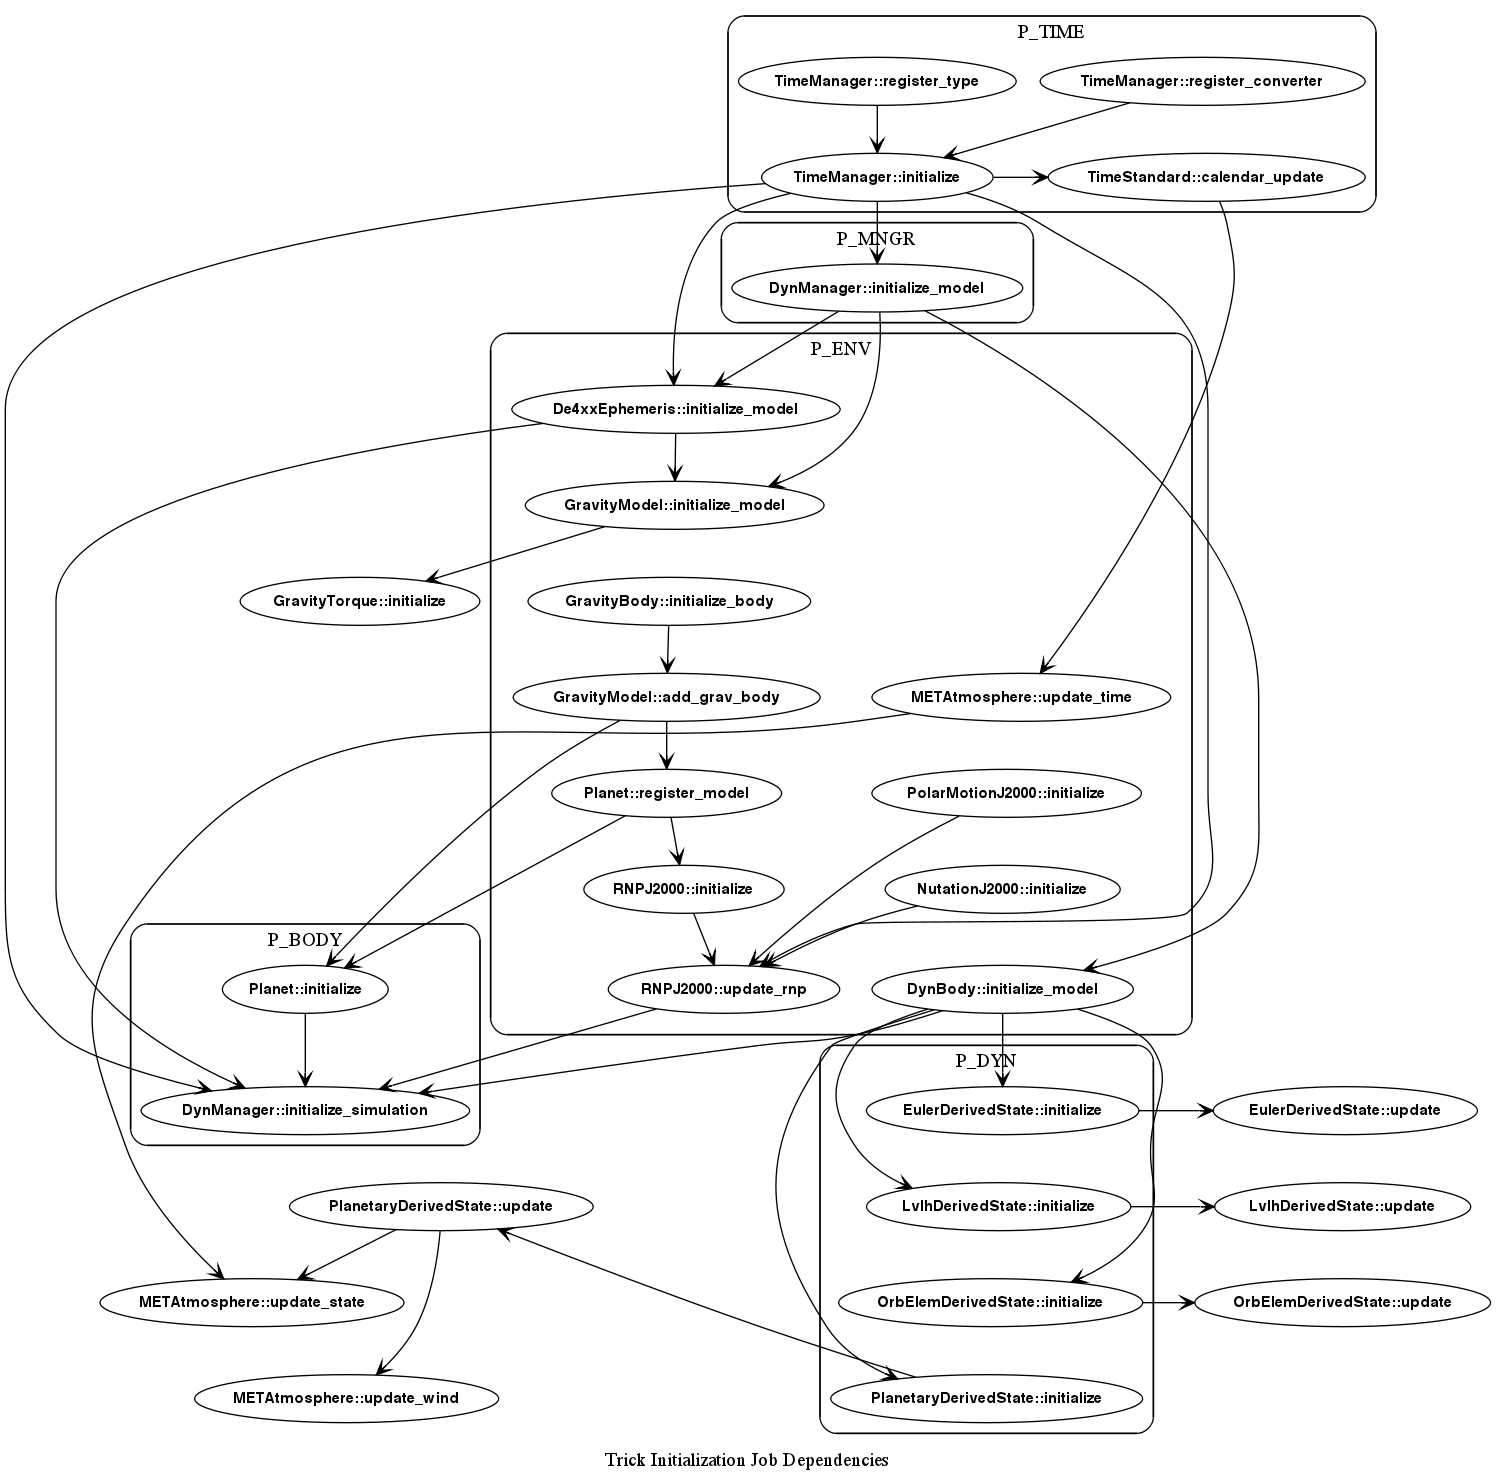
\includegraphics [height=7in]{figs/phasing/initialization.png}
\caption{SIM\_dyncomp job initialization. ERROR - the Planet::initialize method
in the P\_BODY box should be in a P\_EPH box.  This error does not affect the
order in which the jobs in this diagram are called.}
\label{fig:init}
\end{figure}

\clearpage
\newpage
\subsection {Derivative job sequencing}
\begin{figure}[h]
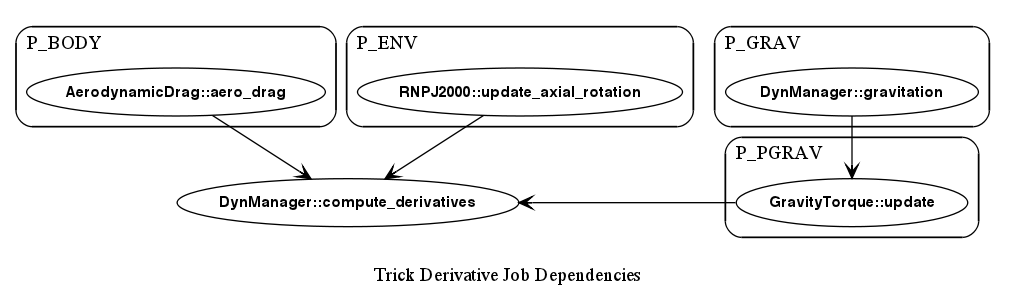
\includegraphics [width=7in]{figs/phasing/derivative.png}
\caption{SIM\_dyncomp derivative job phasing.}
\label{fig:deriv}
\end{figure}

\clearpage
\newpage
\subsection {Scheduled job sequencing}
\begin{figure}[h]
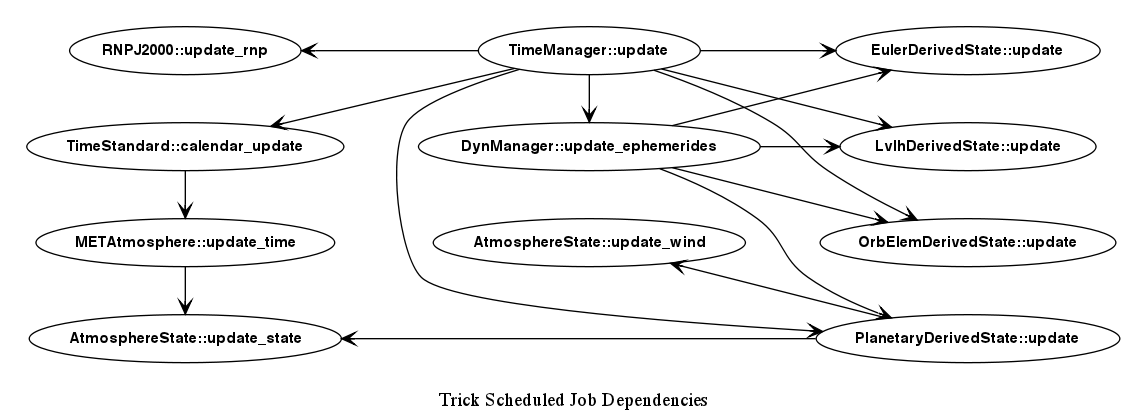
\includegraphics [width=7in]{figs/phasing/scheduled.png}
\caption{SIM\_dyncomp scheduled job phasing.}
\label{fig:sched}
\end{figure}
